\documentclass[1p]{elsarticle_modified}
%\bibliographystyle{elsarticle-num}

%\usepackage[colorlinks]{hyperref}
%\usepackage{abbrmath_seonhwa} %\Abb, \Ascr, \Acal ,\Abf, \Afrak
\usepackage{amsfonts}
\usepackage{amssymb}
\usepackage{amsmath}
\usepackage{amsthm}
\usepackage{scalefnt}
\usepackage{amsbsy}
\usepackage{kotex}
\usepackage{caption}
\usepackage{subfig}
\usepackage{color}
\usepackage{graphicx}
\usepackage{xcolor} %% white, black, red, green, blue, cyan, magenta, yellow
\usepackage{float}
\usepackage{setspace}
\usepackage{hyperref}

\usepackage{tikz}
\usetikzlibrary{arrows}

\usepackage{multirow}
\usepackage{array} % fixed length table
\usepackage{hhline}

%%%%%%%%%%%%%%%%%%%%%
\makeatletter
\renewcommand*\env@matrix[1][\arraystretch]{%
	\edef\arraystretch{#1}%
	\hskip -\arraycolsep
	\let\@ifnextchar\new@ifnextchar
	\array{*\c@MaxMatrixCols c}}
\makeatother %https://tex.stackexchange.com/questions/14071/how-can-i-increase-the-line-spacing-in-a-matrix
%%%%%%%%%%%%%%%

\usepackage[normalem]{ulem}

\newcommand{\msout}[1]{\ifmmode\text{\sout{\ensuremath{#1}}}\else\sout{#1}\fi}
%SOURCE: \msout is \stkout macro in https://tex.stackexchange.com/questions/20609/strikeout-in-math-mode

\newcommand{\cancel}[1]{
	\ifmmode
	{\color{red}\msout{#1}}
	\else
	{\color{red}\sout{#1}}
	\fi
}

\newcommand{\add}[1]{
	{\color{blue}\uwave{#1}}
}

\newcommand{\replace}[2]{
	\ifmmode
	{\color{red}\msout{#1}}{\color{blue}\uwave{#2}}
	\else
	{\color{red}\sout{#1}}{\color{blue}\uwave{#2}}
	\fi
}

\newcommand{\Sol}{\mathcal{S}} %segment
\newcommand{\D}{D} %diagram
\newcommand{\A}{\mathcal{A}} %arc


%%%%%%%%%%%%%%%%%%%%%%%%%%%%%5 test

\def\sl{\operatorname{\textup{SL}}(2,\Cbb)}
\def\psl{\operatorname{\textup{PSL}}(2,\Cbb)}
\def\quan{\mkern 1mu \triangleright \mkern 1mu}

\theoremstyle{definition}
\newtheorem{thm}{Theorem}[section]
\newtheorem{prop}[thm]{Proposition}
\newtheorem{lem}[thm]{Lemma}
\newtheorem{ques}[thm]{Question}
\newtheorem{cor}[thm]{Corollary}
\newtheorem{defn}[thm]{Definition}
\newtheorem{exam}[thm]{Example}
\newtheorem{rmk}[thm]{Remark}
\newtheorem{alg}[thm]{Algorithm}

\newcommand{\I}{\sqrt{-1}}
\begin{document}

%\begin{frontmatter}
%
%\title{Boundary parabolic representations of knots up to 8 crossings}
%
%%% Group authors per affiliation:
%\author{Yunhi Cho} 
%\address{Department of Mathematics, University of Seoul, Seoul, Korea}
%\ead{yhcho@uos.ac.kr}
%
%
%\author{Seonhwa Kim} %\fnref{s_kim}}
%\address{Center for Geometry and Physics, Institute for Basic Science, Pohang, 37673, Korea}
%\ead{ryeona17@ibs.re.kr}
%
%\author{Hyuk Kim}
%\address{Department of Mathematical Sciences, Seoul National University, Seoul 08826, Korea}
%\ead{hyukkim@snu.ac.kr}
%
%\author{Seokbeom Yoon}
%\address{Department of Mathematical Sciences, Seoul National University, Seoul, 08826,  Korea}
%\ead{sbyoon15@snu.ac.kr}
%
%\begin{abstract}
%We find all boundary parabolic representation of knots up to 8 crossings.
%
%\end{abstract}
%\begin{keyword}
%    \MSC[2010] 57M25 
%\end{keyword}
%
%\end{frontmatter}

%\linenumbers
%\tableofcontents
%
\newcommand\colored[1]{\textcolor{white}{\rule[-0.35ex]{0.8em}{1.4ex}}\kern-0.8em\color{red} #1}%
%\newcommand\colored[1]{\textcolor{white}{ #1}\kern-2.17ex	\textcolor{white}{ #1}\kern-1.81ex	\textcolor{white}{ #1}\kern-2.15ex\color{red}#1	}

{\Large $\underline{11n_{154}~(K11n_{154})}$}

\setlength{\tabcolsep}{10pt}
\renewcommand{\arraystretch}{1.6}
\vspace{1cm}\begin{tabular}{m{100pt}>{\centering\arraybackslash}m{274pt}}
\multirow{5}{120pt}{
	\centering
	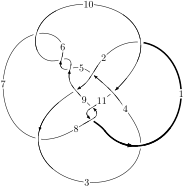
\includegraphics[width=112pt]{../../../GIT/diagram.site/Diagrams/png/770_11n_154.png}\\
\ \ \ A knot diagram\footnotemark}&
\allowdisplaybreaks
\textbf{Linearized knot diagam} \\
\cline{2-2}
 &
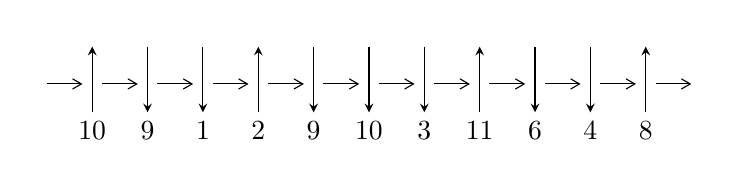
\begin{tikzpicture}[x=20pt, y=17pt]
	% nodes
	\node (C0) at (0, 0) {};
	\node (C1) at (1, 0) {};
	\node (C1U) at (1, +1) {};
	\node (C1D) at (1, -1) {10};

	\node (C2) at (2, 0) {};
	\node (C2U) at (2, +1) {};
	\node (C2D) at (2, -1) {9};

	\node (C3) at (3, 0) {};
	\node (C3U) at (3, +1) {};
	\node (C3D) at (3, -1) {1};

	\node (C4) at (4, 0) {};
	\node (C4U) at (4, +1) {};
	\node (C4D) at (4, -1) {2};

	\node (C5) at (5, 0) {};
	\node (C5U) at (5, +1) {};
	\node (C5D) at (5, -1) {9};

	\node (C6) at (6, 0) {};
	\node (C6U) at (6, +1) {};
	\node (C6D) at (6, -1) {10};

	\node (C7) at (7, 0) {};
	\node (C7U) at (7, +1) {};
	\node (C7D) at (7, -1) {3};

	\node (C8) at (8, 0) {};
	\node (C8U) at (8, +1) {};
	\node (C8D) at (8, -1) {11};

	\node (C9) at (9, 0) {};
	\node (C9U) at (9, +1) {};
	\node (C9D) at (9, -1) {6};

	\node (C10) at (10, 0) {};
	\node (C10U) at (10, +1) {};
	\node (C10D) at (10, -1) {4};

	\node (C11) at (11, 0) {};
	\node (C11U) at (11, +1) {};
	\node (C11D) at (11, -1) {8};
	\node (C12) at (12, 0) {};

	% arrows
	\draw[->,>={angle 60}]
	(C0) edge (C1) (C1) edge (C2) (C2) edge (C3) (C3) edge (C4) (C4) edge (C5) (C5) edge (C6) (C6) edge (C7) (C7) edge (C8) (C8) edge (C9) (C9) edge (C10) (C10) edge (C11) (C11) edge (C12) ;	\draw[->,>=stealth]
	(C1D) edge (C1U) (C2U) edge (C2D) (C3U) edge (C3D) (C4D) edge (C4U) (C5U) edge (C5D) (C6U) edge (C6D) (C7U) edge (C7D) (C8D) edge (C8U) (C9U) edge (C9D) (C10U) edge (C10D) (C11D) edge (C11U) ;
	\end{tikzpicture} \\
\hhline{~~} \\& 
\textbf{Solving Sequence} \\ \cline{2-2} 
 &
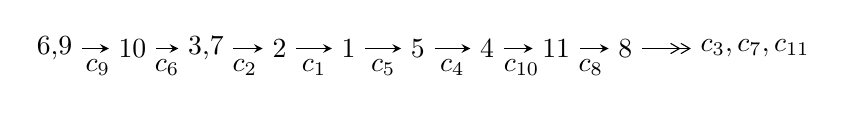
\begin{tikzpicture}[x=25pt, y=7pt]
	% node
	\node (A0) at (-1/8, 0) {6,9};
	\node (A1) at (1, 0) {10};
	\node (A2) at (33/16, 0) {3,7};
	\node (A3) at (25/8, 0) {2};
	\node (A4) at (33/8, 0) {1};
	\node (A5) at (41/8, 0) {5};
	\node (A6) at (49/8, 0) {4};
	\node (A7) at (57/8, 0) {11};
	\node (A8) at (65/8, 0) {8};
	\node (C1) at (1/2, -1) {$c_{9}$};
	\node (C2) at (3/2, -1) {$c_{6}$};
	\node (C3) at (21/8, -1) {$c_{2}$};
	\node (C4) at (29/8, -1) {$c_{1}$};
	\node (C5) at (37/8, -1) {$c_{5}$};
	\node (C6) at (45/8, -1) {$c_{4}$};
	\node (C7) at (53/8, -1) {$c_{10}$};
	\node (C8) at (61/8, -1) {$c_{8}$};
	\node (A9) at (10, 0) {$c_{3},c_{7},c_{11}$};

	% edge
	\draw[->,>=stealth]	
	(A0) edge (A1) (A1) edge (A2) (A2) edge (A3) (A3) edge (A4) (A4) edge (A5) (A5) edge (A6) (A6) edge (A7) (A7) edge (A8) ;
	\draw[->>,>={angle 60}]	
	(A8) edge (A9);
\end{tikzpicture} \\ 

\end{tabular} \\

\footnotetext{
The image of knot diagram is generated by the software ``\textbf{Draw programme}" developed by Andrew Bartholomew(\url{http://www.layer8.co.uk/maths/draw/index.htm\#Running-draw}), where we modified some parts for our purpose(\url{https://github.com/CATsTAILs/LinksPainter}).
}\phantom \\ \newline 
\centering \textbf{Ideals for irreducible components\footnotemark of $X_{\text{par}}$} 
 
\begin{align*}
I^u_{1}&=\langle 
1.31566\times10^{70} u^{49}+5.59358\times10^{70} u^{48}+\cdots+6.53231\times10^{69} b-5.03553\times10^{70},\\
\phantom{I^u_{1}}&\phantom{= \langle  }-3.55956\times10^{70} u^{49}-1.50298\times10^{71} u^{48}+\cdots+6.53231\times10^{69} a+1.72500\times10^{71},\;u^{50}+4 u^{49}+\cdots-6 u+1\rangle \\
I^u_{2}&=\langle 
u^{10}- u^9-3 u^8+3 u^7+4 u^6-4 u^5-7 u^4+6 u^3+7 u^2+b-3 u-2,\\
\phantom{I^u_{2}}&\phantom{= \langle  }-15 u^{10}+10 u^9+45 u^8-26 u^7-61 u^6+30 u^5+107 u^4-44 u^3-102 u^2+a+7 u+21,\\
\phantom{I^u_{2}}&\phantom{= \langle  }u^{11}- u^{10}-3 u^9+3 u^8+4 u^7-4 u^6-7 u^5+6 u^4+7 u^3-4 u^2-2 u+1\rangle \\
\\
\end{align*}
\raggedright * 2 irreducible components of $\dim_{\mathbb{C}}=0$, with total 61 representations.\\
\footnotetext{All coefficients of polynomials are rational numbers. But the coefficients are sometimes approximated in decimal forms when there is not enough margin.}
\newpage
\renewcommand{\arraystretch}{1}
\centering \section*{I. $I^u_{1}= \langle 1.32\times10^{70} u^{49}+5.59\times10^{70} u^{48}+\cdots+6.53\times10^{69} b-5.04\times10^{70},\;-3.56\times10^{70} u^{49}-1.50\times10^{71} u^{48}+\cdots+6.53\times10^{69} a+1.73\times10^{71},\;u^{50}+4 u^{49}+\cdots-6 u+1 \rangle$}
\flushleft \textbf{(i) Arc colorings}\\
\begin{tabular}{m{7pt} m{180pt} m{7pt} m{180pt} }
\flushright $a_{6}=$&$\begin{pmatrix}0\\u\end{pmatrix}$ \\
\flushright $a_{9}=$&$\begin{pmatrix}1\\0\end{pmatrix}$ \\
\flushright $a_{10}=$&$\begin{pmatrix}1\\u^2\end{pmatrix}$ \\
\flushright $a_{3}=$&$\begin{pmatrix}5.44916 u^{49}+23.0084 u^{48}+\cdots+36.9971 u-26.4072\\-2.01408 u^{49}-8.56295 u^{48}+\cdots-15.0392 u+7.70865\end{pmatrix}$ \\
\flushright $a_{7}=$&$\begin{pmatrix}- u\\- u^3+u\end{pmatrix}$ \\
\flushright $a_{2}=$&$\begin{pmatrix}3.43508 u^{49}+14.4454 u^{48}+\cdots+21.9578 u-18.6986\\-2.01408 u^{49}-8.56295 u^{48}+\cdots-15.0392 u+7.70865\end{pmatrix}$ \\
\flushright $a_{1}=$&$\begin{pmatrix}5.50930 u^{49}+23.2971 u^{48}+\cdots+37.7925 u-27.1123\\-1.94686 u^{49}-8.15972 u^{48}+\cdots-13.7847 u+7.15385\end{pmatrix}$ \\
\flushright $a_{5}=$&$\begin{pmatrix}u\\u\end{pmatrix}$ \\
\flushright $a_{4}=$&$\begin{pmatrix}7.20223 u^{49}+30.4910 u^{48}+\cdots+55.1926 u-32.3223\\-1.16935 u^{49}-5.08349 u^{48}+\cdots-12.3880 u+5.64687\end{pmatrix}$ \\
\flushright $a_{11}=$&$\begin{pmatrix}-0.0754028 u^{49}-0.252955 u^{48}+\cdots+13.1088 u+4.21868\\1.44659 u^{49}+5.86887 u^{48}+\cdots+6.37477 u-5.35313\end{pmatrix}$ \\
\flushright $a_{8}=$&$\begin{pmatrix}6.55926 u^{49}+27.8864 u^{48}+\cdots+49.0350 u-30.2341\\-1.23352 u^{49}-5.24956 u^{48}+\cdots-10.3413 u+5.39025\end{pmatrix}$\\ \flushright $a_{8}=$&$\begin{pmatrix}6.55926 u^{49}+27.8864 u^{48}+\cdots+49.0350 u-30.2341\\-1.23352 u^{49}-5.24956 u^{48}+\cdots-10.3413 u+5.39025\end{pmatrix}$\\&\end{tabular}
\flushleft \textbf{(ii) Obstruction class $= -1$}\\~\\
\flushleft \textbf{(iii) Cusp Shapes $= 6.39014 u^{49}+28.2211 u^{48}+\cdots+72.9518 u-36.4279$}\\~\\
\newpage\renewcommand{\arraystretch}{1}
\flushleft \textbf{(iv) u-Polynomials at the component}\newline \\
\begin{tabular}{m{50pt}|m{274pt}}
Crossings & \hspace{64pt}u-Polynomials at each crossing \\
\hline $$\begin{aligned}c_{1}\end{aligned}$$&$\begin{aligned}
&u^{50}+8 u^{49}+\cdots-87 u+71
\end{aligned}$\\
\hline $$\begin{aligned}c_{2}\end{aligned}$$&$\begin{aligned}
&u^{50}+2 u^{49}+\cdots+314 u+193
\end{aligned}$\\
\hline $$\begin{aligned}c_{3}\end{aligned}$$&$\begin{aligned}
&u^{50}-6 u^{49}+\cdots+10 u-1
\end{aligned}$\\
\hline $$\begin{aligned}c_{4}\end{aligned}$$&$\begin{aligned}
&u^{50}-5 u^{49}+\cdots+304 u+403
\end{aligned}$\\
\hline $$\begin{aligned}c_{5},c_{6},c_{9}\end{aligned}$$&$\begin{aligned}
&u^{50}+4 u^{49}+\cdots-6 u+1
\end{aligned}$\\
\hline $$\begin{aligned}c_{7}\end{aligned}$$&$\begin{aligned}
&u^{50}+u^{49}+\cdots+512 u+29
\end{aligned}$\\
\hline $$\begin{aligned}c_{8},c_{11}\end{aligned}$$&$\begin{aligned}
&u^{50}+u^{49}+\cdots+3 u^2+1
\end{aligned}$\\
\hline $$\begin{aligned}c_{10}\end{aligned}$$&$\begin{aligned}
&u^{50}+2 u^{49}+\cdots+13 u-1
\end{aligned}$\\
\hline
\end{tabular}\\~\\
\newpage\renewcommand{\arraystretch}{1}
\flushleft \textbf{(v) Riley Polynomials at the component}\newline \\
\begin{tabular}{m{50pt}|m{274pt}}
Crossings & \hspace{64pt}Riley Polynomials at each crossing \\
\hline $$\begin{aligned}c_{1}\end{aligned}$$&$\begin{aligned}
&y^{50}-20 y^{49}+\cdots-590053 y+5041
\end{aligned}$\\
\hline $$\begin{aligned}c_{2}\end{aligned}$$&$\begin{aligned}
&y^{50}+46 y^{49}+\cdots+780712 y+37249
\end{aligned}$\\
\hline $$\begin{aligned}c_{3}\end{aligned}$$&$\begin{aligned}
&y^{50}-4 y^{49}+\cdots-154 y^2+1
\end{aligned}$\\
\hline $$\begin{aligned}c_{4}\end{aligned}$$&$\begin{aligned}
&y^{50}-45 y^{49}+\cdots-1305446 y+162409
\end{aligned}$\\
\hline $$\begin{aligned}c_{5},c_{6},c_{9}\end{aligned}$$&$\begin{aligned}
&y^{50}-12 y^{49}+\cdots-48 y+1
\end{aligned}$\\
\hline $$\begin{aligned}c_{7}\end{aligned}$$&$\begin{aligned}
&y^{50}+13 y^{49}+\cdots-327684 y+841
\end{aligned}$\\
\hline $$\begin{aligned}c_{8},c_{11}\end{aligned}$$&$\begin{aligned}
&y^{50}+31 y^{49}+\cdots+6 y+1
\end{aligned}$\\
\hline $$\begin{aligned}c_{10}\end{aligned}$$&$\begin{aligned}
&y^{50}-2 y^{49}+\cdots-35 y+1
\end{aligned}$\\
\hline
\end{tabular}\\~\\
\newpage\flushleft \textbf{(vi) Complex Volumes and Cusp Shapes}
$$\begin{array}{c|c|c}  
\text{Solutions to }I^u_{1}& \I (\text{vol} + \sqrt{-1}CS) & \text{Cusp shape}\\
 \hline 
\begin{aligned}
u &= -0.973898 + 0.287950 I \\
a &= -0.695696 + 0.419798 I \\
b &= -0.457776 + 0.369939 I\end{aligned}
 & -1.86387 + 0.30095 I & -9.64984 - 1.90143 I \\ \hline\begin{aligned}
u &= -0.973898 - 0.287950 I \\
a &= -0.695696 - 0.419798 I \\
b &= -0.457776 - 0.369939 I\end{aligned}
 & -1.86387 - 0.30095 I & -9.64984 + 1.90143 I \\ \hline\begin{aligned}
u &= \phantom{-}0.913846 + 0.185540 I \\
a &= -0.335931 + 0.804509 I \\
b &= \phantom{-}0.922990 - 0.289493 I\end{aligned}
 & -2.08438 - 2.77960 I & -10.17164 + 4.44197 I \\ \hline\begin{aligned}
u &= \phantom{-}0.913846 - 0.185540 I \\
a &= -0.335931 - 0.804509 I \\
b &= \phantom{-}0.922990 + 0.289493 I\end{aligned}
 & -2.08438 + 2.77960 I & -10.17164 - 4.44197 I \\ \hline\begin{aligned}
u &= -0.835381 + 0.772928 I \\
a &= \phantom{-}0.47188 + 1.50692 I \\
b &= \phantom{-}0.98491 - 1.67790 I\end{aligned}
 & \phantom{-}2.93158 + 5.78038 I & -3.00000 - 8.73361 I \\ \hline\begin{aligned}
u &= -0.835381 - 0.772928 I \\
a &= \phantom{-}0.47188 - 1.50692 I \\
b &= \phantom{-}0.98491 + 1.67790 I\end{aligned}
 & \phantom{-}2.93158 - 5.78038 I & -3.00000 + 8.73361 I \\ \hline\begin{aligned}
u &= -0.597674 + 0.996526 I \\
a &= -0.095278 - 0.867392 I \\
b &= -0.19400 + 1.85191 I\end{aligned}
 & \phantom{-}0.94420 + 4.84658 I & \phantom{-0.000000 } 0. - 16.7858 I \\ \hline\begin{aligned}
u &= -0.597674 - 0.996526 I \\
a &= -0.095278 + 0.867392 I \\
b &= -0.19400 - 1.85191 I\end{aligned}
 & \phantom{-}0.94420 - 4.84658 I & \phantom{-0.000000 -}0. + 16.7858 I \\ \hline\begin{aligned}
u &= -0.815937 + 0.186566 I \\
a &= \phantom{-}0.64349 - 1.28176 I \\
b &= -0.673813 + 1.147990 I\end{aligned}
 & -4.23706 - 3.34809 I & -10.42134 + 1.19861 I \\ \hline\begin{aligned}
u &= -0.815937 - 0.186566 I \\
a &= \phantom{-}0.64349 + 1.28176 I \\
b &= -0.673813 - 1.147990 I\end{aligned}
 & -4.23706 + 3.34809 I & -10.42134 - 1.19861 I\\
 \hline 
 \end{array}$$\newpage$$\begin{array}{c|c|c}  
\text{Solutions to }I^u_{1}& \I (\text{vol} + \sqrt{-1}CS) & \text{Cusp shape}\\
 \hline 
\begin{aligned}
u &= -0.963408 + 0.692141 I \\
a &= \phantom{-}1.132490 + 0.483149 I \\
b &= -0.25869 - 1.55132 I\end{aligned}
 & \phantom{-}2.51794 - 0.16160 I & \phantom{-0.000000 } 0 \\ \hline\begin{aligned}
u &= -0.963408 - 0.692141 I \\
a &= \phantom{-}1.132490 - 0.483149 I \\
b &= -0.25869 + 1.55132 I\end{aligned}
 & \phantom{-}2.51794 + 0.16160 I & \phantom{-0.000000 } 0 \\ \hline\begin{aligned}
u &= -0.636888 + 1.050190 I \\
a &= \phantom{-}0.675338 + 1.117000 I \\
b &= \phantom{-}0.329148 - 1.016950 I\end{aligned}
 & \phantom{-}3.30459 + 1.24081 I & \phantom{-0.000000 } 0 \\ \hline\begin{aligned}
u &= -0.636888 - 1.050190 I \\
a &= \phantom{-}0.675338 - 1.117000 I \\
b &= \phantom{-}0.329148 + 1.016950 I\end{aligned}
 & \phantom{-}3.30459 - 1.24081 I & \phantom{-0.000000 } 0 \\ \hline\begin{aligned}
u &= \phantom{-}0.903142 + 0.837436 I \\
a &= -0.89244 + 1.30977 I \\
b &= -0.35436 - 1.78012 I\end{aligned}
 & \phantom{-}4.40850 - 3.12436 I & \phantom{-0.000000 } 0 \\ \hline\begin{aligned}
u &= \phantom{-}0.903142 - 0.837436 I \\
a &= -0.89244 - 1.30977 I \\
b &= -0.35436 + 1.78012 I\end{aligned}
 & \phantom{-}4.40850 + 3.12436 I & \phantom{-0.000000 } 0 \\ \hline\begin{aligned}
u &= -0.557299 + 0.500566 I \\
a &= -1.78993 + 1.80158 I \\
b &= \phantom{-}0.421947 - 0.110229 I\end{aligned}
 & -3.04563 + 6.16036 I & -5.83312 - 10.36352 I \\ \hline\begin{aligned}
u &= -0.557299 - 0.500566 I \\
a &= -1.78993 - 1.80158 I \\
b &= \phantom{-}0.421947 + 0.110229 I\end{aligned}
 & -3.04563 - 6.16036 I & -5.83312 + 10.36352 I \\ \hline\begin{aligned}
u &= -0.736164\phantom{ +0.000000I} \\
a &= -0.886089\phantom{ +0.000000I} \\
b &= -0.812664\phantom{ +0.000000I}\end{aligned}
 & -1.37116\phantom{ +0.000000I} & -7.85670\phantom{ +0.000000I} \\ \hline\begin{aligned}
u &= -0.288799 + 0.670270 I \\
a &= -0.549822 + 0.201160 I \\
b &= -0.231209 + 0.384240 I\end{aligned}
 & -0.74993 + 1.80678 I & -3.40421 - 3.27437 I\\
 \hline 
 \end{array}$$\newpage$$\begin{array}{c|c|c}  
\text{Solutions to }I^u_{1}& \I (\text{vol} + \sqrt{-1}CS) & \text{Cusp shape}\\
 \hline 
\begin{aligned}
u &= -0.288799 - 0.670270 I \\
a &= -0.549822 - 0.201160 I \\
b &= -0.231209 - 0.384240 I\end{aligned}
 & -0.74993 - 1.80678 I & -3.40421 + 3.27437 I \\ \hline\begin{aligned}
u &= \phantom{-}0.710444 + 0.074039 I \\
a &= \phantom{-}1.60904 - 1.03329 I \\
b &= \phantom{-}1.205030 - 0.316628 I\end{aligned}
 & -4.51765 + 4.23526 I & -12.34564 - 0.73227 I \\ \hline\begin{aligned}
u &= \phantom{-}0.710444 - 0.074039 I \\
a &= \phantom{-}1.60904 + 1.03329 I \\
b &= \phantom{-}1.205030 + 0.316628 I\end{aligned}
 & -4.51765 - 4.23526 I & -12.34564 + 0.73227 I \\ \hline\begin{aligned}
u &= \phantom{-}0.965620 + 0.857282 I \\
a &= -0.820961 + 1.063210 I \\
b &= -0.18244 - 1.58681 I\end{aligned}
 & \phantom{-}4.33842 - 3.23438 I & \phantom{-0.000000 } 0 \\ \hline\begin{aligned}
u &= \phantom{-}0.965620 - 0.857282 I \\
a &= -0.820961 - 1.063210 I \\
b &= -0.18244 + 1.58681 I\end{aligned}
 & \phantom{-}4.33842 + 3.23438 I & \phantom{-0.000000 } 0 \\ \hline\begin{aligned}
u &= \phantom{-}0.563185 + 0.349209 I \\
a &= \phantom{-}0.166277 + 0.562597 I \\
b &= -2.08804 - 0.12116 I\end{aligned}
 & -3.78607 - 5.93938 I & -6.42894 + 12.06653 I \\ \hline\begin{aligned}
u &= \phantom{-}0.563185 - 0.349209 I \\
a &= \phantom{-}0.166277 - 0.562597 I \\
b &= -2.08804 + 0.12116 I\end{aligned}
 & -3.78607 + 5.93938 I & -6.42894 - 12.06653 I \\ \hline\begin{aligned}
u &= \phantom{-}0.802008 + 1.081440 I \\
a &= \phantom{-}0.618176 - 0.851982 I \\
b &= \phantom{-}0.02927 + 1.60011 I\end{aligned}
 & \phantom{-}6.57814 + 2.00021 I & \phantom{-0.000000 } 0 \\ \hline\begin{aligned}
u &= \phantom{-}0.802008 - 1.081440 I \\
a &= \phantom{-}0.618176 + 0.851982 I \\
b &= \phantom{-}0.02927 - 1.60011 I\end{aligned}
 & \phantom{-}6.57814 - 2.00021 I & \phantom{-0.000000 } 0 \\ \hline\begin{aligned}
u &= -0.790681 + 1.114590 I \\
a &= -0.805915 - 0.850484 I \\
b &= \phantom{-}0.14947 + 1.53184 I\end{aligned}
 & \phantom{-}3.11102 - 8.02113 I & \phantom{-0.000000 } 0\\
 \hline 
 \end{array}$$\newpage$$\begin{array}{c|c|c}  
\text{Solutions to }I^u_{1}& \I (\text{vol} + \sqrt{-1}CS) & \text{Cusp shape}\\
 \hline 
\begin{aligned}
u &= -0.790681 - 1.114590 I \\
a &= -0.805915 + 0.850484 I \\
b &= \phantom{-}0.14947 - 1.53184 I\end{aligned}
 & \phantom{-}3.11102 + 8.02113 I & \phantom{-0.000000 } 0 \\ \hline\begin{aligned}
u &= -0.292603 + 0.539944 I \\
a &= \phantom{-}0.367718 + 0.535422 I \\
b &= \phantom{-}0.956495 + 0.240511 I\end{aligned}
 & \phantom{-}1.06170 + 1.95789 I & \phantom{-}2.50049 - 3.97543 I \\ \hline\begin{aligned}
u &= -0.292603 - 0.539944 I \\
a &= \phantom{-}0.367718 - 0.535422 I \\
b &= \phantom{-}0.956495 - 0.240511 I\end{aligned}
 & \phantom{-}1.06170 - 1.95789 I & \phantom{-}2.50049 + 3.97543 I \\ \hline\begin{aligned}
u &= \phantom{-}0.549411 + 0.272810 I \\
a &= \phantom{-}0.49144 + 2.18390 I \\
b &= -0.042142 - 0.459151 I\end{aligned}
 & -0.60147 - 2.63277 I & \phantom{-}0.64260 + 6.35036 I \\ \hline\begin{aligned}
u &= \phantom{-}0.549411 - 0.272810 I \\
a &= \phantom{-}0.49144 - 2.18390 I \\
b &= -0.042142 + 0.459151 I\end{aligned}
 & -0.60147 + 2.63277 I & \phantom{-}0.64260 - 6.35036 I \\ \hline\begin{aligned}
u &= -1.40477\phantom{ +0.000000I} \\
a &= -0.402422\phantom{ +0.000000I} \\
b &= -0.427165\phantom{ +0.000000I}\end{aligned}
 & -2.53971\phantom{ +0.000000I} & \phantom{-0.000000 } 0 \\ \hline\begin{aligned}
u &= -1.030240 + 0.960055 I \\
a &= -0.435587 - 0.666622 I \\
b &= -0.65359 + 1.43821 I\end{aligned}
 & -0.48592 + 3.61316 I & \phantom{-0.000000 } 0 \\ \hline\begin{aligned}
u &= -1.030240 - 0.960055 I \\
a &= -0.435587 + 0.666622 I \\
b &= -0.65359 - 1.43821 I\end{aligned}
 & -0.48592 - 3.61316 I & \phantom{-0.000000 } 0 \\ \hline\begin{aligned}
u &= \phantom{-}0.91934 + 1.08476 I \\
a &= -0.616459 + 1.203170 I \\
b &= -0.238685 - 1.355140 I\end{aligned}
 & \phantom{-}4.11263 - 3.83167 I & \phantom{-0.000000 } 0 \\ \hline\begin{aligned}
u &= \phantom{-}0.91934 - 1.08476 I \\
a &= -0.616459 - 1.203170 I \\
b &= -0.238685 + 1.355140 I\end{aligned}
 & \phantom{-}4.11263 + 3.83167 I & \phantom{-0.000000 } 0\\
 \hline 
 \end{array}$$\newpage$$\begin{array}{c|c|c}  
\text{Solutions to }I^u_{1}& \I (\text{vol} + \sqrt{-1}CS) & \text{Cusp shape}\\
 \hline 
\begin{aligned}
u &= \phantom{-}1.11330 + 0.90983 I \\
a &= \phantom{-}0.632047 - 0.971558 I \\
b &= \phantom{-}0.65462 + 1.62579 I\end{aligned}
 & \phantom{-}5.57747 - 9.21703 I & \phantom{-0.000000 } 0 \\ \hline\begin{aligned}
u &= \phantom{-}1.11330 - 0.90983 I \\
a &= \phantom{-}0.632047 + 0.971558 I \\
b &= \phantom{-}0.65462 - 1.62579 I\end{aligned}
 & \phantom{-}5.57747 + 9.21703 I & \phantom{-0.000000 } 0 \\ \hline\begin{aligned}
u &= -1.12578 + 0.90724 I \\
a &= -0.566919 - 1.147900 I \\
b &= -0.72405 + 1.73806 I\end{aligned}
 & \phantom{-}2.0157 + 15.3090 I & \phantom{-0.000000 } 0 \\ \hline\begin{aligned}
u &= -1.12578 - 0.90724 I \\
a &= -0.566919 + 1.147900 I \\
b &= -0.72405 - 1.73806 I\end{aligned}
 & \phantom{-}2.0157 - 15.3090 I & \phantom{-0.000000 } 0 \\ \hline\begin{aligned}
u &= -1.21156 + 0.89742 I \\
a &= \phantom{-}0.397984 + 0.889144 I \\
b &= \phantom{-}0.173869 - 1.329530 I\end{aligned}
 & \phantom{-}1.55527 + 5.89362 I & \phantom{-0.000000 } 0 \\ \hline\begin{aligned}
u &= -1.21156 - 0.89742 I \\
a &= \phantom{-}0.397984 - 0.889144 I \\
b &= \phantom{-}0.173869 + 1.329530 I\end{aligned}
 & \phantom{-}1.55527 - 5.89362 I & \phantom{-0.000000 } 0 \\ \hline\begin{aligned}
u &= \phantom{-}1.51600 + 0.17015 I \\
a &= \phantom{-}0.324411 + 0.071542 I \\
b &= -0.043698 - 0.329284 I\end{aligned}
 & -7.03500 - 5.35259 I & \phantom{-0.000000 } 0 \\ \hline\begin{aligned}
u &= \phantom{-}1.51600 - 0.17015 I \\
a &= \phantom{-}0.324411 - 0.071542 I \\
b &= -0.043698 + 0.329284 I\end{aligned}
 & -7.03500 + 5.35259 I & \phantom{-0.000000 } 0 \\ \hline\begin{aligned}
u &= \phantom{-}0.234313 + 0.025877 I \\
a &= -3.28109 + 3.13603 I \\
b &= -0.065339 - 0.963971 I\end{aligned}
 & \phantom{-}0.24228 - 2.13866 I & -2.49155 + 4.03852 I \\ \hline\begin{aligned}
u &= \phantom{-}0.234313 - 0.025877 I \\
a &= -3.28109 - 3.13603 I \\
b &= -0.065339 + 0.963971 I\end{aligned}
 & \phantom{-}0.24228 + 2.13866 I & -2.49155 - 4.03852 I\\
 \hline 
 \end{array}$$\newpage\newpage\renewcommand{\arraystretch}{1}
\centering \section*{II. $I^u_{2}= \langle u^{10}- u^9+\cdots+b-2,\;-15 u^{10}+10 u^9+\cdots+a+21,\;u^{11}- u^{10}+\cdots-2 u+1 \rangle$}
\flushleft \textbf{(i) Arc colorings}\\
\begin{tabular}{m{7pt} m{180pt} m{7pt} m{180pt} }
\flushright $a_{6}=$&$\begin{pmatrix}0\\u\end{pmatrix}$ \\
\flushright $a_{9}=$&$\begin{pmatrix}1\\0\end{pmatrix}$ \\
\flushright $a_{10}=$&$\begin{pmatrix}1\\u^2\end{pmatrix}$ \\
\flushright $a_{3}=$&$\begin{pmatrix}15 u^{10}-10 u^9+\cdots-7 u-21\\- u^{10}+u^9+3 u^8-3 u^7-4 u^6+4 u^5+7 u^4-6 u^3-7 u^2+3 u+2\end{pmatrix}$ \\
\flushright $a_{7}=$&$\begin{pmatrix}- u\\- u^3+u\end{pmatrix}$ \\
\flushright $a_{2}=$&$\begin{pmatrix}14 u^{10}-9 u^9+\cdots-4 u-19\\- u^{10}+u^9+3 u^8-3 u^7-4 u^6+4 u^5+7 u^4-6 u^3-7 u^2+3 u+2\end{pmatrix}$ \\
\flushright $a_{1}=$&$\begin{pmatrix}20 u^{10}-14 u^9+\cdots-11 u-26\\u^{10}- u^9-2 u^8+2 u^7+2 u^6-2 u^5-5 u^4+4 u^3+2 u^2- u+1\end{pmatrix}$ \\
\flushright $a_{5}=$&$\begin{pmatrix}u\\u\end{pmatrix}$ \\
\flushright $a_{4}=$&$\begin{pmatrix}-21 u^{10}+10 u^9+\cdots- u+42\\-10 u^{10}+6 u^9+\cdots+3 u+16\end{pmatrix}$ \\
\flushright $a_{11}=$&$\begin{pmatrix}13 u^{10}-11 u^9+\cdots-15 u-16\\8 u^{10}-5 u^9+\cdots-2 u-14\end{pmatrix}$ \\
\flushright $a_{8}=$&$\begin{pmatrix}-19 u^{10}+10 u^9+\cdots-148 u^2+35\\-6 u^{10}+3 u^9+\cdots- u+10\end{pmatrix}$\\ \flushright $a_{8}=$&$\begin{pmatrix}-19 u^{10}+10 u^9+\cdots-148 u^2+35\\-6 u^{10}+3 u^9+\cdots- u+10\end{pmatrix}$\\&\end{tabular}
\flushleft \textbf{(ii) Obstruction class $= 1$}\\~\\
\flushleft \textbf{(iii) Cusp Shapes $= 37 u^{10}-17 u^9-120 u^8+48 u^7+172 u^6-57 u^5-289 u^4+70 u^3+294 u^2+3 u-78$}\\~\\
\newpage\renewcommand{\arraystretch}{1}
\flushleft \textbf{(iv) u-Polynomials at the component}\newline \\
\begin{tabular}{m{50pt}|m{274pt}}
Crossings & \hspace{64pt}u-Polynomials at each crossing \\
\hline $$\begin{aligned}c_{1}\end{aligned}$$&$\begin{aligned}
&u^{11}+u^{10}- u^9-4 u^8+u^6-2 u^5-3 u^4+3 u^3+2 u^2- u-1
\end{aligned}$\\
\hline $$\begin{aligned}c_{2}\end{aligned}$$&$\begin{aligned}
&u^{11}+u^{10}+2 u^9+4 u^8-2 u^7+u^6-2 u^5-9 u^4+9 u^3+2 u^2-4 u+1
\end{aligned}$\\
\hline $$\begin{aligned}c_{3}\end{aligned}$$&$\begin{aligned}
&u^{11}+5 u^{10}+\cdots+4 u+1
\end{aligned}$\\
\hline $$\begin{aligned}c_{4}\end{aligned}$$&$\begin{aligned}
&u^{11}-6 u^{10}+\cdots+4 u-1
\end{aligned}$\\
\hline $$\begin{aligned}c_{5},c_{6}\end{aligned}$$&$\begin{aligned}
&u^{11}+u^{10}-3 u^9-3 u^8+4 u^7+4 u^6-7 u^5-6 u^4+7 u^3+4 u^2-2 u-1
\end{aligned}$\\
\hline $$\begin{aligned}c_{7}\end{aligned}$$&$\begin{aligned}
&u^{11}+2 u^{10}+5 u^9+9 u^8+9 u^7+2 u^6+5 u^5+12 u^4+10 u^3-2 u-1
\end{aligned}$\\
\hline $$\begin{aligned}c_{8}\end{aligned}$$&$\begin{aligned}
&u^{11}+4 u^9-2 u^8+6 u^7-8 u^6+u^5-13 u^4-4 u^3-7 u^2-2 u-1
\end{aligned}$\\
\hline $$\begin{aligned}c_{9}\end{aligned}$$&$\begin{aligned}
&u^{11}- u^{10}-3 u^9+3 u^8+4 u^7-4 u^6-7 u^5+6 u^4+7 u^3-4 u^2-2 u+1
\end{aligned}$\\
\hline $$\begin{aligned}c_{10}\end{aligned}$$&$\begin{aligned}
&u^{11}+u^{10}-2 u^9-3 u^8+3 u^7+2 u^6- u^5+4 u^3+u^2- u-1
\end{aligned}$\\
\hline $$\begin{aligned}c_{11}\end{aligned}$$&$\begin{aligned}
&u^{11}+4 u^9+2 u^8+6 u^7+8 u^6+u^5+13 u^4-4 u^3+7 u^2-2 u+1
\end{aligned}$\\
\hline
\end{tabular}\\~\\
\newpage\renewcommand{\arraystretch}{1}
\flushleft \textbf{(v) Riley Polynomials at the component}\newline \\
\begin{tabular}{m{50pt}|m{274pt}}
Crossings & \hspace{64pt}Riley Polynomials at each crossing \\
\hline $$\begin{aligned}c_{1}\end{aligned}$$&$\begin{aligned}
&y^{11}-3 y^{10}+\cdots+5 y-1
\end{aligned}$\\
\hline $$\begin{aligned}c_{2}\end{aligned}$$&$\begin{aligned}
&y^{11}+3 y^{10}+\cdots+12 y-1
\end{aligned}$\\
\hline $$\begin{aligned}c_{3}\end{aligned}$$&$\begin{aligned}
&y^{11}-3 y^{10}+\cdots+20 y^2-1
\end{aligned}$\\
\hline $$\begin{aligned}c_{4}\end{aligned}$$&$\begin{aligned}
&y^{11}-4 y^{10}+18 y^8+40 y^7+28 y^6+45 y^5+75 y^4+70 y^3+5 y^2-6 y-1
\end{aligned}$\\
\hline $$\begin{aligned}c_{5},c_{6},c_{9}\end{aligned}$$&$\begin{aligned}
&y^{11}-7 y^{10}+\cdots+12 y-1
\end{aligned}$\\
\hline $$\begin{aligned}c_{7}\end{aligned}$$&$\begin{aligned}
&y^{11}+6 y^{10}+\cdots+4 y-1
\end{aligned}$\\
\hline $$\begin{aligned}c_{8},c_{11}\end{aligned}$$&$\begin{aligned}
&y^{11}+8 y^{10}+\cdots-10 y-1
\end{aligned}$\\
\hline $$\begin{aligned}c_{10}\end{aligned}$$&$\begin{aligned}
&y^{11}-5 y^{10}+\cdots+3 y-1
\end{aligned}$\\
\hline
\end{tabular}\\~\\
\newpage\flushleft \textbf{(vi) Complex Volumes and Cusp Shapes}
$$\begin{array}{c|c|c}  
\text{Solutions to }I^u_{2}& \I (\text{vol} + \sqrt{-1}CS) & \text{Cusp shape}\\
 \hline 
\begin{aligned}
u &= -0.775260 + 0.879276 I \\
a &= \phantom{-}0.187286 + 0.932840 I \\
b &= \phantom{-}0.21109 - 1.51914 I\end{aligned}
 & \phantom{-}0.70704 + 4.35639 I & -5.54956 - 2.55288 I \\ \hline\begin{aligned}
u &= -0.775260 - 0.879276 I \\
a &= \phantom{-}0.187286 - 0.932840 I \\
b &= \phantom{-}0.21109 + 1.51914 I\end{aligned}
 & \phantom{-}0.70704 - 4.35639 I & -5.54956 + 2.55288 I \\ \hline\begin{aligned}
u &= -0.780915 + 0.043107 I \\
a &= \phantom{-}0.35176 + 1.37931 I \\
b &= -0.495745 - 0.113579 I\end{aligned}
 & -1.14703 + 2.08475 I & -5.67789 + 0.04134 I \\ \hline\begin{aligned}
u &= -0.780915 - 0.043107 I \\
a &= \phantom{-}0.35176 - 1.37931 I \\
b &= -0.495745 + 0.113579 I\end{aligned}
 & -1.14703 - 2.08475 I & -5.67789 - 0.04134 I \\ \hline\begin{aligned}
u &= \phantom{-}0.874107 + 0.934732 I \\
a &= -0.74222 + 1.34614 I \\
b &= -0.34039 - 1.50546 I\end{aligned}
 & \phantom{-}3.59148 - 3.42396 I & -7.58514 + 2.00100 I \\ \hline\begin{aligned}
u &= \phantom{-}0.874107 - 0.934732 I \\
a &= -0.74222 - 1.34614 I \\
b &= -0.34039 + 1.50546 I\end{aligned}
 & \phantom{-}3.59148 + 3.42396 I & -7.58514 - 2.00100 I \\ \hline\begin{aligned}
u &= \phantom{-}1.380430 + 0.112956 I \\
a &= \phantom{-}0.051000 + 0.348587 I \\
b &= -0.660833 - 0.171838 I\end{aligned}
 & -7.66458 - 5.46030 I & -13.6502 + 4.8917 I \\ \hline\begin{aligned}
u &= \phantom{-}1.380430 - 0.112956 I \\
a &= \phantom{-}0.051000 - 0.348587 I \\
b &= -0.660833 + 0.171838 I\end{aligned}
 & -7.66458 + 5.46030 I & -13.6502 - 4.8917 I \\ \hline\begin{aligned}
u &= -1.42602\phantom{ +0.000000I} \\
a &= \phantom{-}0.376679\phantom{ +0.000000I} \\
b &= \phantom{-}0.724774\phantom{ +0.000000I}\end{aligned}
 & -2.78763\phantom{ +0.000000I} & -26.4320\phantom{ +0.000000I} \\ \hline\begin{aligned}
u &= \phantom{-}0.514652 + 0.025908 I \\
a &= \phantom{-}0.96384 + 2.00148 I \\
b &= \phantom{-}1.42350 - 0.12348 I\end{aligned}
 & -3.96271 - 5.00716 I & -8.32130 + 5.65788 I\\
 \hline 
 \end{array}$$\newpage$$\begin{array}{c|c|c}  
\text{Solutions to }I^u_{2}& \I (\text{vol} + \sqrt{-1}CS) & \text{Cusp shape}\\
 \hline 
\begin{aligned}
u &= \phantom{-}0.514652 - 0.025908 I \\
a &= \phantom{-}0.96384 - 2.00148 I \\
b &= \phantom{-}1.42350 + 0.12348 I\end{aligned}
 & -3.96271 + 5.00716 I & -8.32130 - 5.65788 I\\
 \hline 
 \end{array}$$\newpage
\newpage\renewcommand{\arraystretch}{1}
\centering \section*{ III. u-Polynomials}
\begin{tabular}{m{50pt}|m{274pt}}
Crossings & \hspace{64pt}u-Polynomials at each crossing \\
\hline $$\begin{aligned}c_{1}\end{aligned}$$&$\begin{aligned}
&(u^{11}+u^{10}- u^9-4 u^8+u^6-2 u^5-3 u^4+3 u^3+2 u^2- u-1)\\
&\cdot(u^{50}+8 u^{49}+\cdots-87 u+71)
\end{aligned}$\\
\hline $$\begin{aligned}c_{2}\end{aligned}$$&$\begin{aligned}
&(u^{11}+u^{10}+2 u^9+4 u^8-2 u^7+u^6-2 u^5-9 u^4+9 u^3+2 u^2-4 u+1)\\
&\cdot(u^{50}+2 u^{49}+\cdots+314 u+193)
\end{aligned}$\\
\hline $$\begin{aligned}c_{3}\end{aligned}$$&$\begin{aligned}
&(u^{11}+5 u^{10}+\cdots+4 u+1)(u^{50}-6 u^{49}+\cdots+10 u-1)
\end{aligned}$\\
\hline $$\begin{aligned}c_{4}\end{aligned}$$&$\begin{aligned}
&(u^{11}-6 u^{10}+\cdots+4 u-1)(u^{50}-5 u^{49}+\cdots+304 u+403)
\end{aligned}$\\
\hline $$\begin{aligned}c_{5},c_{6}\end{aligned}$$&$\begin{aligned}
&(u^{11}+u^{10}-3 u^9-3 u^8+4 u^7+4 u^6-7 u^5-6 u^4+7 u^3+4 u^2-2 u-1)\\
&\cdot(u^{50}+4 u^{49}+\cdots-6 u+1)
\end{aligned}$\\
\hline $$\begin{aligned}c_{7}\end{aligned}$$&$\begin{aligned}
&(u^{11}+2 u^{10}+5 u^9+9 u^8+9 u^7+2 u^6+5 u^5+12 u^4+10 u^3-2 u-1)\\
&\cdot(u^{50}+u^{49}+\cdots+512 u+29)
\end{aligned}$\\
\hline $$\begin{aligned}c_{8}\end{aligned}$$&$\begin{aligned}
&(u^{11}+4 u^9-2 u^8+6 u^7-8 u^6+u^5-13 u^4-4 u^3-7 u^2-2 u-1)\\
&\cdot(u^{50}+u^{49}+\cdots+3 u^2+1)
\end{aligned}$\\
\hline $$\begin{aligned}c_{9}\end{aligned}$$&$\begin{aligned}
&(u^{11}- u^{10}-3 u^9+3 u^8+4 u^7-4 u^6-7 u^5+6 u^4+7 u^3-4 u^2-2 u+1)\\
&\cdot(u^{50}+4 u^{49}+\cdots-6 u+1)
\end{aligned}$\\
\hline $$\begin{aligned}c_{10}\end{aligned}$$&$\begin{aligned}
&(u^{11}+u^{10}-2 u^9-3 u^8+3 u^7+2 u^6- u^5+4 u^3+u^2- u-1)\\
&\cdot(u^{50}+2 u^{49}+\cdots+13 u-1)
\end{aligned}$\\
\hline $$\begin{aligned}c_{11}\end{aligned}$$&$\begin{aligned}
&(u^{11}+4 u^9+2 u^8+6 u^7+8 u^6+u^5+13 u^4-4 u^3+7 u^2-2 u+1)\\
&\cdot(u^{50}+u^{49}+\cdots+3 u^2+1)
\end{aligned}$\\
\hline
\end{tabular}\newpage\renewcommand{\arraystretch}{1}
\centering \section*{ IV. Riley Polynomials}
\begin{tabular}{m{50pt}|m{274pt}}
Crossings & \hspace{64pt}Riley Polynomials at each crossing \\
\hline $$\begin{aligned}c_{1}\end{aligned}$$&$\begin{aligned}
&(y^{11}-3 y^{10}+\cdots+5 y-1)(y^{50}-20 y^{49}+\cdots-590053 y+5041)
\end{aligned}$\\
\hline $$\begin{aligned}c_{2}\end{aligned}$$&$\begin{aligned}
&(y^{11}+3 y^{10}+\cdots+12 y-1)(y^{50}+46 y^{49}+\cdots+780712 y+37249)
\end{aligned}$\\
\hline $$\begin{aligned}c_{3}\end{aligned}$$&$\begin{aligned}
&(y^{11}-3 y^{10}+\cdots+20 y^2-1)(y^{50}-4 y^{49}+\cdots-154 y^2+1)
\end{aligned}$\\
\hline $$\begin{aligned}c_{4}\end{aligned}$$&$\begin{aligned}
&(y^{11}-4 y^{10}+18 y^8+40 y^7+28 y^6+45 y^5+75 y^4+70 y^3+5 y^2-6 y-1)\\
&\cdot(y^{50}-45 y^{49}+\cdots-1305446 y+162409)
\end{aligned}$\\
\hline $$\begin{aligned}c_{5},c_{6},c_{9}\end{aligned}$$&$\begin{aligned}
&(y^{11}-7 y^{10}+\cdots+12 y-1)(y^{50}-12 y^{49}+\cdots-48 y+1)
\end{aligned}$\\
\hline $$\begin{aligned}c_{7}\end{aligned}$$&$\begin{aligned}
&(y^{11}+6 y^{10}+\cdots+4 y-1)(y^{50}+13 y^{49}+\cdots-327684 y+841)
\end{aligned}$\\
\hline $$\begin{aligned}c_{8},c_{11}\end{aligned}$$&$\begin{aligned}
&(y^{11}+8 y^{10}+\cdots-10 y-1)(y^{50}+31 y^{49}+\cdots+6 y+1)
\end{aligned}$\\
\hline $$\begin{aligned}c_{10}\end{aligned}$$&$\begin{aligned}
&(y^{11}-5 y^{10}+\cdots+3 y-1)(y^{50}-2 y^{49}+\cdots-35 y+1)
\end{aligned}$\\
\hline
\end{tabular}
\vskip 2pc
\end{document}